\documentclass[10pt]{article}
\usepackage[margin=18mm]{geometry}
\usepackage{graphicx,booktabs}
\setlength{\parskip}{0.6em}
\begin{document}
\section*{Abstract and research question}
\subsection*{Response Process Analysis for Assessment Review}
Group 04 | Machine Learning Applications | Le Hoang The Quyen, Tran Gia Thanh and Nguyen Phu Trong

\subsection*{Abstract}
We studied whether response times and selection actions add predictive information after recent correctness is observed. Five outer participant folds covered 995 adults and 9,950 development windows. Adding time to logistic regression changed pooled log loss by -0.002861. The gain was small relative to the contribution of score history. Action features showed an uncertain additional gain on log loss. These estimates describe an exploratory reanalysis of one assessment protocol.

\subsection*{Problem and intended use}
An assessment designer deciding whether to retain or review response logs needs to know when those logs improve a forecast based on scores. We estimate the probability of fewer than two correct answers on the next three items. The evidence applies to adults completing this fixed matrix-reasoning protocol. Classroom decisions, psychological diagnoses and intervention effects require separate evidence.

\subsection*{Relation to the source study}
Much et al. [1] released response, duration and action data collected for validation of psychometric models of speed and persistence. Group 04 defines a prospective information boundary within each block and compares predictive probabilities across feature sets and model families. The original preregistration concerns the source study.

\clearpage
\section*{Data and methods}
\subsection*{Source, permission and input selection}
Much et al. [1, 2] released data for 1,244 adults under CC BY 4.0. The authors replaced Prolific IDs with study-generated numeric IDs [1, sections 3.6-3.7]. With --release Data, Code/01\_prepare\_data.py verifies the three original CSVs and writes the MR01-MR20 response, action and key fields to Data/source/. The main and supplemental codebooks define these fields.

\subsection*{Measurement and participant boundaries}
Code/02\_build\_features.py replays ordered toggles, checks X\_MR selections and Y\_MR scores against the key, and matches T\_MR milliseconds to final-submit cumulTime, including 41 repeated-submit pairs. Of 24,880 records, 143 blank scores were verified as omissions and counted as zero. Invalid times fail the audit. Valid long durations and all 232 zero-score participants are retained.

Stage 02 validates Results/splits/, sets aside 249 test participants and writes 9,950 windows for 995 people to Results/features/development\_windows.csv. Each person's blocks stay in one outer fold. Stage 03 tunes on three inner participant folds recorded in Results/fit/inner\_folds.csv.

\subsection*{Prediction time}
After item j = 3 through 7, the event is fewer than two correct among the next three items. Only completed items in the current block supply responses, times and actions. Future correctness supplies the label. Final scores and post-study disruptions are excluded.

\subsection*{One development prediction}
ID 2096, block 1, anchor 7 had recent correctness 0, 1, 0 and durations 20.528, 30.187 and 95.493 seconds. The history prior predicted 0.8281, Outcomes LR 0.6346 and Combined LR 0.4406. The next three items were all correct, giving label zero. This is a held-out fold prediction.

\subsection*{Features and baselines}
The history prior estimates a smoothed event rate per recent correct count. Outcomes LR distinguishes the most recent score, recent-three accuracy, completed-prefix accuracy and known block/anchor/instruction context. Combined LR adds latest, recent and prefix log(1 + seconds). Relative timing centers log time by training-item medians and completed person history. Process LR adds recent toggle counts, deselection fractions and first-action latencies.

\clearpage
\section*{Experimental setup and overall results}
All observations for one person stay together. Of 1,244 participants, 249 belonged to a previously examined historical test cohort. The reconstruction excludes them from model fitting, tuning and evaluation. Five outer folds hold out 199 people each. Three inner folds select by pooled log loss. Encoders, scalers and item medians are fitted on each training fold. All LR variants share one model family.

LR tunes C over 0.1 and 1.0. The reconstructed LR standardizes the full encoded matrix. CART uses Gini impurity, depths 3, 5 or 8, and minimum leaf sizes 20 or 50. CART uses the same inner assignments and feature sets. Model and fold seeds are 42. The score-only versus score-plus-time comparison changes one feature set while preserving evaluation units.

\noindent\textbf{Table 1. Development out-of-fold metrics}\par
\begin{tabular}{llll}
\toprule
Model & Log loss & Brier & AUC \\
\midrule
History prior & 0.330964 & 0.105886 & 0.908955 \\
Outcomes LR & 0.307811 & 0.098606 & 0.931279 \\
Combined LR & 0.304950 & 0.097459 & 0.933109 \\
Process LR & 0.303345 & 0.096760 & 0.933799 \\
Combined CART & 0.313132 & 0.099607 & 0.924953 \\
Process CART & 0.312967 & 0.099675 & 0.924587 \\
\bottomrule
\end{tabular}

Lower log loss and Brier score indicate better probability estimates. AUC measures ranking. Compare the two LR rows to isolate the timing increment. Combined CART has higher log loss than Combined LR for the declared tuning grid.

\noindent\textbf{Table 2. Paired log-loss differences, first model minus second}\par
\begin{tabular}{lllll}
\toprule
Scope & First & Second & Difference & 95\% interval \\
\midrule
all & Outcomes LR & History prior & -0.023153 & [-0.029271, -0.016931] \\
all & Combined LR & Outcomes LR & -0.002861 & [-0.005526, -0.000247] \\
all & Process LR & Combined LR & -0.001605 & [-0.003375, +0.000145] \\
all & Combined CART & Combined LR & +0.008182 & [+0.003605, +0.012901] \\
\bottomrule
\end{tabular}

Intervals use 2,000 paired participant-bootstrap draws, seed 2026. They condition on fitted predictions and omit refitting uncertainty. Comparisons use exploratory, unadjusted intervals.

\clearpage
\section*{Timing across recent score histories}
\noindent\textbf{Table 3. Counts and log loss by recent correctness}\par
\begin{tabular}{lllllll}
\toprule
Recent & People & Windows & Events & Others & Scores & + Time \\
\midrule
0/3 & 610 & 4165 & 4127 & 38 & 0.042110 & 0.042943 \\
1/3 & 576 & 1456 & 1210 & 246 & 0.409452 & 0.401148 \\
2/3 & 569 & 1803 & 810 & 993 & 0.649046 & 0.642688 \\
3/3 & 499 & 2526 & 440 & 2086 & 0.443760 & 0.440441 \\
\bottomrule
\end{tabular}

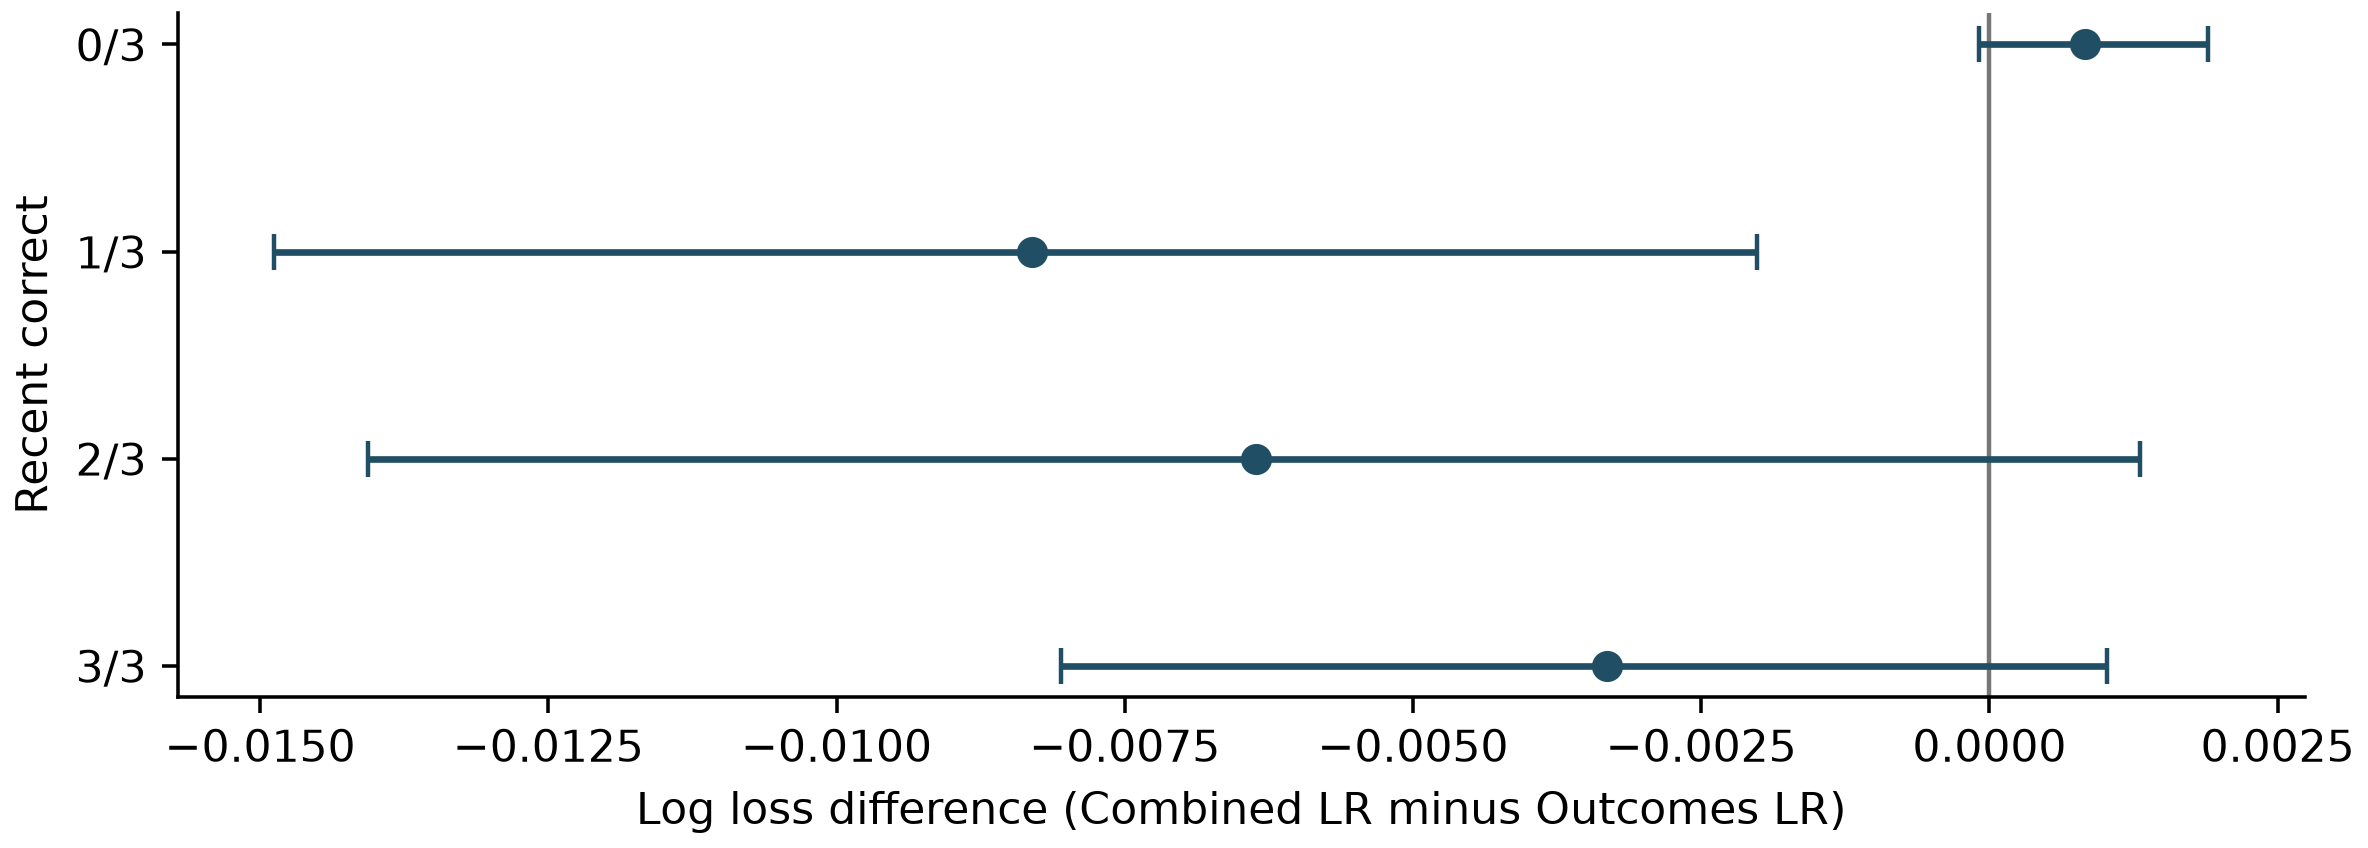
\includegraphics[width=\linewidth]{../Results/figures/timing_by_history.png}
Figure 1. Timing increment in log loss with paired participant intervals.

At 0/3 there are 4,127 events and 38 non-events. Adding time worsens the point estimate, but its interval includes zero. AUC alone describes ranking against a small exceptional class; log loss penalizes confident errors. A common timing coefficient could contribute to the pattern. This mechanism has not been established. For pooled 1/3 and 2/3, the difference is -0.007228 [-0.012818, -0.001421]. This focus followed feedback and was exploratory.

Replacing raw timing with relative timing gives an overall difference of +0.000021 [-0.000040, +0.000078]. The evidence does not establish a general incremental advantage for centering or action summaries. People can appear in multiple history groups.

\clearpage
\section*{Error analysis and review workload}
Within the 1/3 history group, rank the signed change (2y - 1) times (p\_combined - p\_outcomes). Take the five largest positive changes and the five most negative. Resolve ties by public ID, block and anchor. The first five rows move toward the observed label. Probabilities concern the future-score event.

\noindent\textbf{Table 4. Selected development cases}\par
\begin{tabular}{lllllll}
\toprule
ID & Block/j & Scores & Recent seconds & Scores p & + Time p & Label \\
\midrule
2096 & 1/7 & 010 & 20.5, 30.2, 95.5 & 0.635 & 0.441 & 0 \\
2787 & 1/6 & 001 & 151.7, 2311.1, 298.0 & 0.670 & 0.858 & 1 \\
2216 & 1/5 & 100 & 178.1, 538.8, 123.7 & 0.719 & 0.885 & 1 \\
1766 & 1/6 & 100 & 115.1, 43.3, 124.7 & 0.671 & 0.837 & 1 \\
2112 & 1/7 & 010 & 33.4, 62.8, 68.2 & 0.638 & 0.489 & 0 \\
1617 & 1/5 & 100 & 17.1, 21.5, 39.1 & 0.755 & 0.543 & 1 \\
1675 & 2/6 & 001 & 198.4, 163.6, 31.0 & 0.514 & 0.698 & 0 \\
3122 & 2/7 & 100 & 18.3, 37.2, 45.3 & 0.756 & 0.582 & 1 \\
3122 & 2/6 & 010 & 14.2, 18.3, 37.2 & 0.531 & 0.371 & 1 \\
1617 & 2/7 & 010 & 10.7, 38.2, 61.9 & 0.738 & 0.586 & 1 \\
\bottomrule
\end{tabular}

These are selected extremes, so they cannot estimate typical benefit. Case-specific observations require inspection of the actual responses and durations. Completed member records: 0 of 10. The separate member register preserves evidence and decisions across reruns.

\noindent\textbf{Table 5. Within-fold review capacity for Combined LR}\par
\begin{tabular}{lllll}
\toprule
Budget & Selected & Events & Precision & Recall \\
\midrule
5\% & 495 & 494 & 0.9980 & 0.0750 \\
10\% & 995 & 993 & 0.9980 & 0.1508 \\
20\% & 1990 & 1987 & 0.9985 & 0.3017 \\
\bottomrule
\end{tabular}

Each fold contributes the floor of its budget times its number of windows. Ties use ID, block and anchor. High precision occurs alongside many missed events; this retrospective ranking has no validated deployment threshold.

\clearpage
\section*{Historical comparison, discussion and conclusion}
\noindent\textbf{Table 6. Original Week 10 and current reconstruction}\par
\begin{tabular}{llll}
\toprule
History & Model & Original log loss & Current log loss \\
\midrule
all & Outcomes LR & 0.307353 & 0.307811 \\
all & Combined LR & 0.305201 & 0.304950 \\
0/3 & Outcomes LR & 0.042152 & 0.042110 \\
0/3 & Combined LR & 0.043581 & 0.042943 \\
1/3 & Outcomes LR & 0.409324 & 0.409452 \\
1/3 & Combined LR & 0.401725 & 0.401148 \\
\bottomrule
\end{tabular}

Both runs use identical raw source files and share the 249 test IDs. They assign only 212 of 995 development participants the same numbered outer fold. The original used ID-sorted outer seed 20261021, inner seed 20261030 plus fold, numeric-only standardization and bootstrap seed 20261024. The reconstruction uses the saved seed-42 assignments and scales the encoded design. Changing bootstrap seeds affects intervals for fixed predictions. The specific contribution of each training difference has not been isolated.

The original 0/3 timing interval excluded zero. The reconstructed interval includes it. Each conclusion must follow its own run. The historical forecasts in Table 6 are recovered from the original saved probabilities. The LR-CART comparison and the ten selected cases use current probabilities.

\subsection*{Discussion and limitations}
The source study frames timing in an experimental assessment setting [1]. Liang [3] examined timing and accuracy in gamified university quizzes. That setting differs in task, participants and feedback. Here, overlapping windows, an English-speaking adult volunteer sample and previously examined development data limit generalization. Action logs measure recorded behavior; they do not establish motive.

\subsection*{Conclusion}
Score history accounts for most of the observed predictive gain. Timing contributes a smaller improvement, particularly in mixed score histories. The additional value of actions and the applicability of these probabilities to other assessments remain uncertain.

\clearpage
\section*{References and reproducibility}
[1] Much, S., Mutak, A., Pohl, S., and Ranger, J. (2025). Data From a Validation Study of Two Psychometric Models on Test-taking Behavior. Journal of Open Psychology Data, 13, 1. DOI 10.5334/jopd.124.

[2] Much, S., Mutak, A., Pohl, S., and Ranger, J. (2024). Modeling speed-ability trade-off and test-taking persistence: Parameter validation for two psychometric models. Open Science Framework. DOI 10.17605/OSF.IO/9J6HM.

[3] Liang, Z. (2024). More haste, less speed? Relationship between response time and response accuracy in gamified online quizzes in an undergraduate engineering course. Frontiers in Education, 9, 1412954. DOI 10.3389/feduc.2024.1412954.

\subsection*{Reproduction and use of AI}
Run the five numbered scripts in Code in order. Results/table\_sources.csv identifies the generators for the analysis tables. Report/report\_sources.csv identifies each displayed table and figure. Data/README.md documents the public release, transformations and license. AI\_Log/AI\_Use\_Log.md records tool assistance and the outstanding individual source or code checks.

\end{document}
